

\documentclass[journal]{IEEEtran}




\usepackage[pdftex]{graphicx}
% \graphicspath{{../pdf/}{../jpeg/}}
% \DeclareGraphicsExtensions{.pdf,.jpeg,.png}
\usepackage{amsmath}
\usepackage{booktabs}
\usepackage{amssymb}
\usepackage{wasysym}
\usepackage{listings}

%\usepackage{algorithmic}
%\usepackage{array}
%\usepackage{url}
% correct bad hyphenation here
\hyphenation{op-tical net-works semi-conduc-tor}

\usepackage{xcolor}
\usepackage{listings}
\lstset{basicstyle=\ttfamily,
	showstringspaces=false,
	commentstyle=\color{red},
	keywordstyle=\color{blue}
}

\usepackage{biblatex}
\usepackage[colorlinks=true,allcolors=black]{hyperref}
%\usepackage[backend=biber, bibencoding=utf8, style=ieee]{biblatex}
\addbibresource{references.bib}






\hyphenation{op-tical net-works semi-conduc-tor}


\begin{document}

\title{Assignment 3 - Phase 2: Using gem5 for estimating the performance of different application mappings onto different multi-core processors
}

\author{Snorri Steffanson, Filippo Bernardi,~\IEEEmembership{Master students,~TU Eindhoven}
}



% The paper headers
\markboth{Using gem5 analize application mapped onto different multi-core processors - S. Steffanson, F. Bernardi}%
{Shell \MakeLowercase{\textit{et al.}}: Bare Demo of IEEEtran.cls for IEEE Journals}


\maketitle

% As a general rule, do not put math, special symbols or citations
% in the abstract or keywords.
\begin{abstract}

\end{abstract}

% Note that keywords are not normally used for peerreview papers.
\begin{IEEEkeywords}
ARM a9, ARM a15, gem5
\end{IEEEkeywords}




\IEEEpeerreviewmaketitle



\section{Introduction}

\IEEEPARstart{T}{his} paper shows performance evaluation of the same application, a jpeg encoder onto two different processors. Those two processors are composed differently. The first is a 3 ARM a9 core CPU. The second has one ARM a15 core and an ARM a9 core on it.
The first step done it was to analyze the given application. For this task, Valgrind program has been used.
The results is shown in figure \ref{fig:valgrind}

\begin{figure}[!h]
	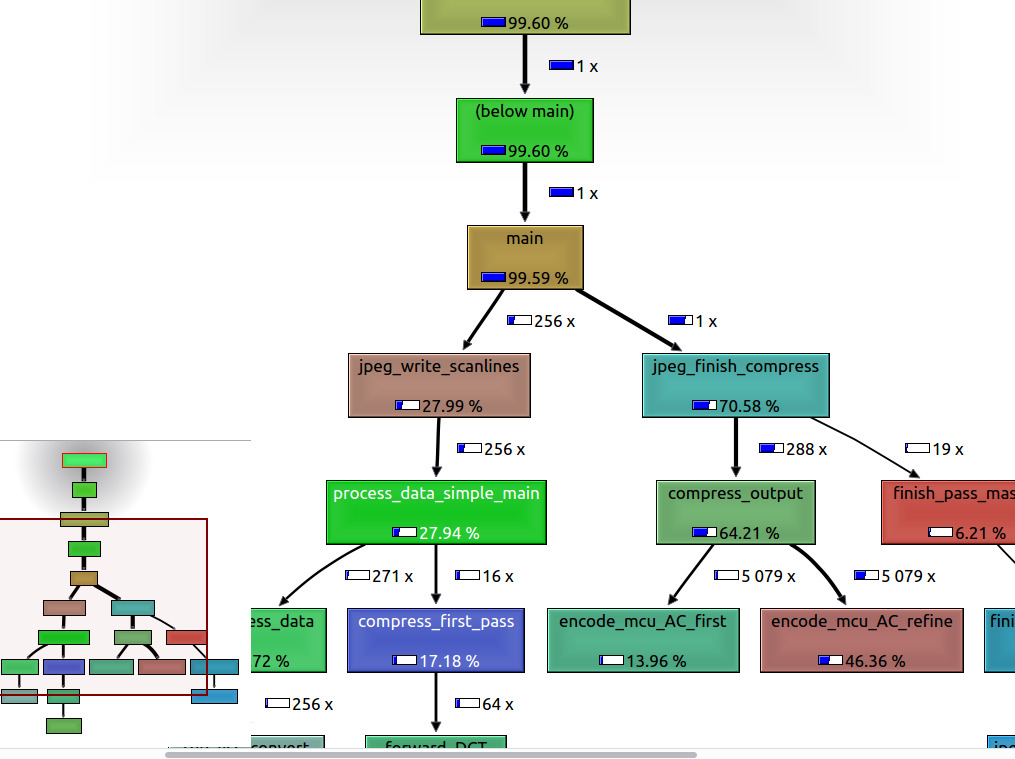
\includegraphics[width=\linewidth]{valgrind}
	\caption{Program calls in Valgrind}
	\label{fig:valgrind}
\end{figure}

This results gives the hint of divide the code inside the CPUs onto different cores, after the main function.\\
 
\hfill January 15, 2017

\section{First Part}

What as been done firstly is try to run on the two architecture without change any code, the results has been the following:
23714598000 number of tick for the 3 a9 cores and 18786430000. 
Now, the jpeg finish compression has been placed in another thread, for doing so the following tutorial has been used: http://timmurphy.org/2010/05/04/pthreads-in-c-a-minimal-working-example/

On one thred the jpeg\_finish\_compress there are the same results for 3 a9 23641697000 and 21533576000 for a15-a9



\section{Second Part}
Due to the complexity of the jpeg compressing function we have decided to change to the same type of application but exploited in a simple manner. The new Program calls tree it can be seen in Figure \ref{fig:valgrind2}

\begin{figure}[!h]
	\centering
	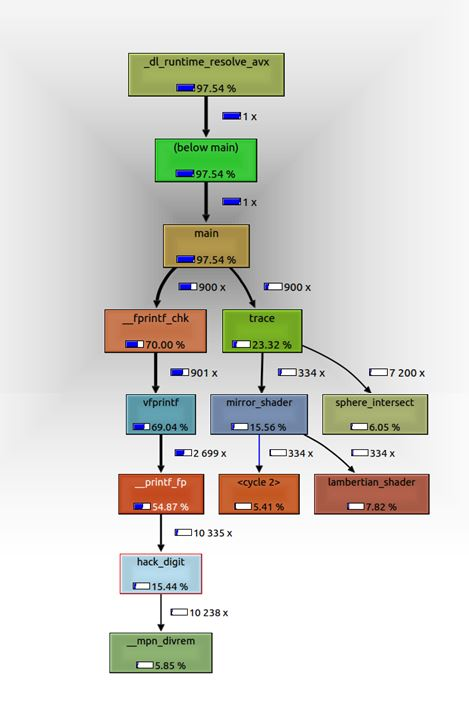
\includegraphics[width=.8\linewidth]{valgrind2}
	\caption{New jpeg application calls in Valgrind}
	\label{fig:valgrind2}
\end{figure}


\section{appendix}
\subsection{scripts}
\begin{lstlisting}
#!/bin/sh
cd /home/$USER/srt-clean
sudo rm callgrind.out.*
valgrind --tool=callgrind ./srt
kcachegrind callgrind.out.*
cd /
\end{lstlisting}

\begin{lstlisting}
#/bin/sh!
cd /home/$USER/srt-clean
make clean
make
cd /
\end{lstlisting}

\begin{lstlisting}
#/bin/sh!
cd /home/$USER/srt-clean
make clean
make -f Makefile.arm
/home/$USER/gem5/build/ARM/gem5.opt
/home/$USER/gem5/configs/example/arm-multic
	ore-A15-A9.py -c
	/home/$USER/srt-clean/srt
cd /
\end{lstlisting}

\begin{lstlisting}
#/bin/sh!
cd /home/$USER/jpeg/jpeg-6a/
make clean
make -f Makefile.arm
/home/$USER/gem5/build/ARM/gem5.opt
	 /home/$USER/gem5/configs/example/
	arm-multicore-A9-A9-A9.py -c 
	/home/$USER/srt-clean/srt
cd /
\end{lstlisting}


\begin{lstlisting}
#/bin/sh!
cd /home/$USER/srt-clean
make clean
make -f Makefile.arm
cd /
\end{lstlisting}



\section{Conclusion}
Conclusion
\end{document}


